
\documentclass[a4paper]{book}
\usepackage{amsfonts}
\usepackage{amsmath}
\usepackage{graphicx}
\usepackage{pythonhighlight}
\usepackage{hyperref}
\title{The Bempp Handbook}
\author{Timo Betcke and Matthew W. Scroggs}
\begin{document}
\maketitle


Welcome to the Bempp Handbook, the main documentation for bempp-cl.
Installation instructions and example problems can be found at
\href{https://bempp.com/documentation}{bempp.com/documentation}, as well as documentation
for the legacy version of Bempp (3.3.4).


\part{Introduction}


The boundary element method (BEM) is a numerical method for approximating the solution of partial differential equations (PDEs).
The method finds the approximation by discretising a boundary integral equation that can be derived from the PDE.

Bempp is an open-source boundary element method library that can be used to assemble all the standard integral kernels for
Laplace, Helmholtz, modified Helmholtz, and Maxwell problems. The library has a user-friendly Python interface that allows the
user to use BEM to solve a variety of problems, including problems in electrostatics, acoustics and electromagnetics.

Bempp began life as BEM++, and was a Python library with a fast C++ computational core. The ++ slowly changed to a pp as
functionality gradually moved from C++ to Python. The latest version, \pyth{bempp-cl}, is a complete rewrite of the library, with
the C++ core replaced by just-in-time compiled OpenCL kernels, and has many improvements over past versions of the library.

Bempp is divided into two parts: \pyth{bempp.api} and \pyth{bempp.core}.
The user interface of the library is contained in \pyth{bempp.api}.
The core assembly routines of the library are contained in \pyth{bempp.core}. The majority of users of Bempp are unlikely to need
to directly interact with the functionality in \pyth{bempp.core}.

In this handbook, we introduce and demonstrate the functionality of Bempp. The handbook is split into three parts.
First, we present \href{api/index.md}{a guide to using Bempp}. This part of the handbook takes the reader
through all the major functionality contained in the \pyth{bempp.api} user interface.

In the second part of the handbook, we take \href{core/index.md}{a journey into the Bempp core} where we look in more detail
at the internal behaviour of the Bempp assemblers

For the final part of the handbook, we present \href{theory/index.md}{a Bempp user's introduction to boundary element methods}.
This part of the handbook aims the introduce the mathematics underlying BEM and highlight important aspects of the
theory that should be taken into account when deciding how to approach BEM problems.

This handbook is hosted on \href{https://github.com/bempp/bempp-handbook}{GitHub} and we welcome suggestions for improving it
in the issues and pull requests.


\part{A Guide to Using Bempp}


This section of the Bempp Handbook gives details of the functionality of Bempp.

The Bempp library is divided into two parts: \pyth{bempp.api} and \pyth{bempp.core}.
The user-friendly functionality of the library is contained in \pyth{bempp.api}, while
the fast computation routines are contained in \pyth{bempp.core}.

In this section we focus on the functionality in \pyth{bempp.api}.


\chapter{Grids}


In order to solve a problem using the boundary element method, we must first define the grid
(or mesh) on which the problem will be discretised.
In Bempp, the grid will be a triangulation of a 2D surface in 3D space.
Bempp currently only supports grids consisting of flat surface triangles.

This section looks at how grids can be created and used in Bempp.


\section{Creating a Grid}


A Bempp grid can be created using a built-in grid, by importing a gmsh file,
or by providing the grid data.

We first import Bempp and NumPy.

\begin{python}
import bempp.api
import numpy as np
\end{python}

\subsection{ Built-in grids}Various shapes are included in the \pyth{bempp.api.shapes} module, and discretisations with
different numbers of elements can be created using these.
In order for the these built-in grids to work, Gmsh must be
installed and the command \pyth{gmsh} must be available in the path.

The command \pyth{regular_sphere} creates a sphere by refining a
base octahedron. The number of elements in the sphere is given by
$8 \times 4^n$, where $n$ is the refinement level.
The following command creates a triangulation of a sphere with refinement level 3:

\begin{python}
grid = bempp.api.shapes.regular_sphere(3)
\end{python}

The command \pyth{sphere} creates a sphere with a chosen element size.
The following command creates a sphere with element diameter $h=0.1$:

\begin{python}
grid = bempp.api.shapes.sphere(h=0.1)
\end{python}

The command \pyth{cube} creates a cube with a chosen element size.
The following command creates a cube with element diameter $h=0.3$:

\begin{python}
grid = bempp.api.shapes.cube(h=0.3)
\end{python}

Full automatically-generated documentation of Bempp's available built-in grids can be found
\href{https://bempp-cl.readthedocs.io/en/latest/docs/bempp/api/shapes/index.html}{here}.

\subsection{ Importing a grid}Grids can be importedusing Bempp's \pyth{import_grid} command.
For example, the following command will load a grid from the Gmsh file \pyth{my_grid.msh}.

\begin{python}
grid = bempp.api.import_grid('my_grid.msh')
\end{python}

Bempp uses the file ending to recognise a number of grid formats.
Importing grids is handled by the \href{https://github.com/nschloe/meshio}{meshio} library.
    
This works through the external \pyth{meshio} library.
A list of all files types that can be imported can be found in the meshio documentation.
Frequently used formats with Bempp are \pyth{.msh} (Gmsh),
\pyth{.vtk} (Legacy VTK), and \pyth{.vtu} (VTK Xml Format).

\subsection{ Creating a grid from element data}Bempp grids can be generated from arrays containing vertex coordinates and
connectivity information. For example, to create a grid consisting of two
triangles with vertices $\{(0, 0, 0), (1, 0, 0), (0, 1, 0)\}$ and
$\{(1, 0, 0), (1, 1, 0), (0, 1, 0)\}$ we use the following commands:

\begin{python}
vertices = np.array(
    [[0, 1, 0, 1], [0, 0, 1, 1], [0, 0, 0, 0]],
    dtype=np.float64)
elements = np.array(
    [[0, 1], [1, 3], [2, 2]], dtype=np.uint32)
grid = bempp.api.Grid(vertices, elements)
\end{python}

Note that the three arrays in the \pyth{vertices} array are the $x$-coordinates,
then the $y$-coordinates, then the $z$-coordinates.
Similarly, the three arrays in the \pyth{elements} array are the first points of each triangle,
then the second points, then the third points.
In general, the \pyth{vertices} and \pyth{elements} arrays should have shapes $3\times M$ and $3\times N$
(respectively) for a grid with $M$ vertices and $N$ elements.

The array \pyth{vertices} contains the 3D coordinates of all vertices. The array
\pyth{elements} contains the connectivity information. In this case the first
triangle consists of the vertices 0, 1, 2, and the second triangle consists
of the vertices 1, 3, 2.

Optionally, we can specify a list \pyth{domain_indices}
that gives different groups of elements the same id. This can be used
for example to generate different types of boundary data on different parts
of the grid, or to specify function spaces only on parts of the grid. In this
example, both triangles automatically have the identifier 0 since nothing
else was specified. This is equivalent to running:

\begin{python}
grid = bempp.api.Grid(vertices, elements, domain_indices=[0, 0])
\end{python}


\section{Working with Grids}

Once you have created a Bempp grid, you may want to use information about your grid.
This page show how commonly used information can be obtained from a Bempp grid.

\subsection{ Querying grid information}
The number of elements, edges and vertices in a grid are given by:

\begin{python}
grid.number_of_elements
grid.number_of_edges
grid.number_of_vertices
\end{python}

To query the maximum and minimum element diameter use the following attributes:

\begin{python}
grid.maximum_element_diameter
grid.minimum_element_diameter
\end{python}

The vertex indices of the element 5 can be obtained using:

\begin{python}
grid.elements[:, 5]
\end{python}

Note that the numbering of element starts at 0, so element 5 is the grid's sixth element.

The vertex coordinates of element 5 can be found using:

\begin{python}
grid.vertices[:, grid.elements[:, 5]]
\end{python}

The area of the element 5 is:

\begin{python}
grid.volumes[5]
\end{python}

The edge indices associated with element 5 are:

\begin{python}
grid.element_edges[5]
\end{python}

The vertex indices of the edges of element 5 can be obtained using:

\begin{python}
grid.edges[:, grid.element_edges[:, 5]]
\end{python}

This returns a 2$\times$3 array of the vertex coordinates associated
with the three edges of the element.
Edges in Bempp are ordered in the following way:

\begin{center}
\begin{tabular}{|l|l|l|}
\hline
Edge & First vertex & Second vertex\\
\hline
 0   &  0           &  1\\
 1   &  0           &  2\\
 2   &  1           &  2\\
\hline
\end{tabular}
\end{center}
Full automatically-generated documentation of the Bempp \pyth{Grid} class can be found
\href{https://bempp-cl.readthedocs.io/en/latest/docs/bempp/api/grid/grid/index.html#bempp.api.grid.grid.Grid}{here}.

\subsection{ Plotting and exporting grids}To export a grid, we can use the \pyth{export} command:

\begin{python}
bempp.api.export('grid.msh', grid=grid)
\end{python}

This commands export the object \pyth{grid} as Gmsh file with the
name \pyth{grid.msh}.

In order to plot a grid, we can simply use the command:

\begin{python}
grid.plot()
\end{python}

By default, this will plot using Gmsh (or plotly if you are inside a Jupyter notebook).
The following command can be used to change the plotting backend.

\begin{python}
bempp.api.PLOT_BACKEND = "gmsh"
bempp.api.PLOT_BACKEND = "paraview"
\end{python}

This requires Gmsh or Paraview to be available in the system path.


\chapter{Function Spaces}


Once we have created a grid, we can define finite-dimensional function spaces
on the grid. These spaces will then be used to discretise the boundary integral
formulations of our problem.


\section{Defining a Function Space}


The function \pyth{function_space} is used to initialise spaces. To define
a space of piecewise constant functions we use the command:

\begin{python}
space = bempp.api.function_space(grid, "DP", 0)
\end{python}

The parameter \pyth{DP} is short for Discontinuous Polynomial. The number 0 is
the degree of the polynomial space. To define a space of continuous, piecewise
linear functions use:

\begin{python}
space = bempp.api.function_space(grid, "P", 1)
\end{python}

Bempp-cl only supports function spaces up to degree 1. This is an important
difference to earlier versions that also supported higher order spaces.

The number of degrees of freedom (DOFs) in a space can be found using:

\begin{python}
space.global_dof_count
\end{python}

For solving Laplace or Helmholtz problems, \href{scalar_spaces.md}{scalar function spaces}
should be used.
For solving Maxwell's equations, \href{vector_spaces.md}{vector function spaces}
should be used.


\section{Scalar Function Spaces}


The following scalar-valued spaces are supported in Bempp:

\begin{center}
\begin{tabular}{|l|l|l|}
\hline
Space Type & Order(s) & Description\\
\hline
\verb@"DP"@     & 0 or 1   & Discontinuous polynomials\\
\verb@"P"@      & 1        & Continuous polynomials\\
\verb@"DUAL"@   & 0 or 1   & Dual spaces on the barycentrically refined grid\\
\hline
\end{tabular}
\end{center}
\subsection{ Discontinuous polynomial spaces}DP spaces are polynomial inside each element and discontinuous between elements.
An example basis function of an order 0 DP space is shown below.

\begin{center}
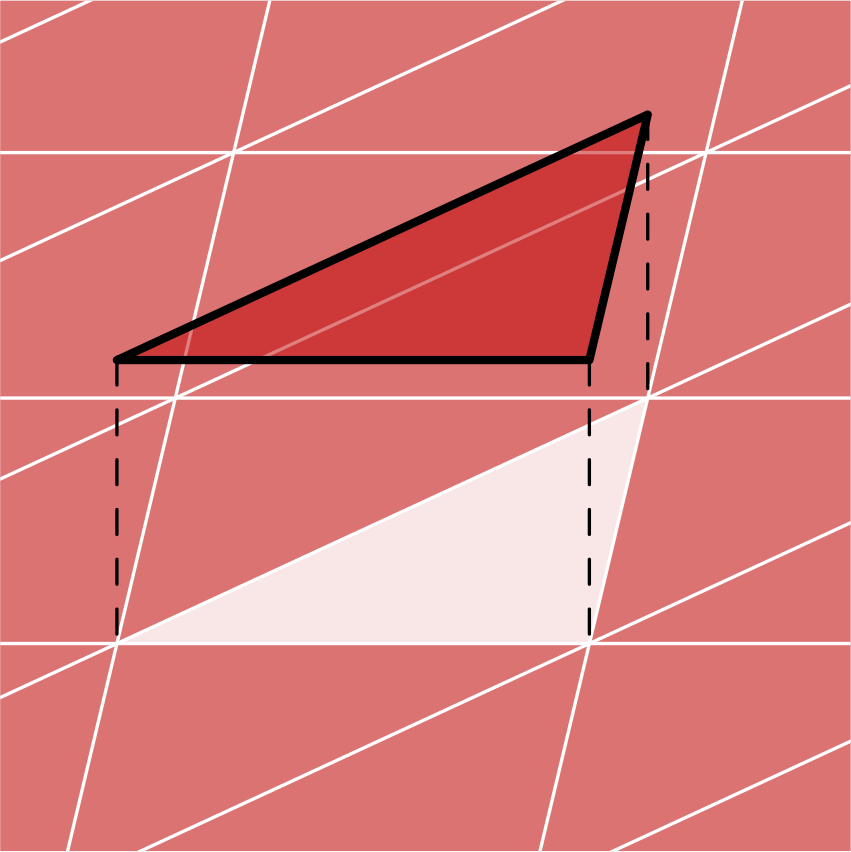
\includegraphics[width=0.6\textwidth]{../img/dp0.png}

\footnotesize{Discontinuous polynomial order 0 basis function}\end{center}

These spaces can be created in Bempp with:

\begin{python}
space = bempp.api.function_space(grid, "DP", 0)
space = bempp.api.function_space(grid, "DP", 1)
\end{python}

The DOFs of an order 0 DP space are at the midpoints of each cell.
The DOFs of an order 1 DP space are at the three vertices of each cell.

\subsection{ Continuous polynomial spaces}P spaces are polynomial inside each element and continuous between elements.
An example basis function of an order 1 P space is shown below.

\begin{center}
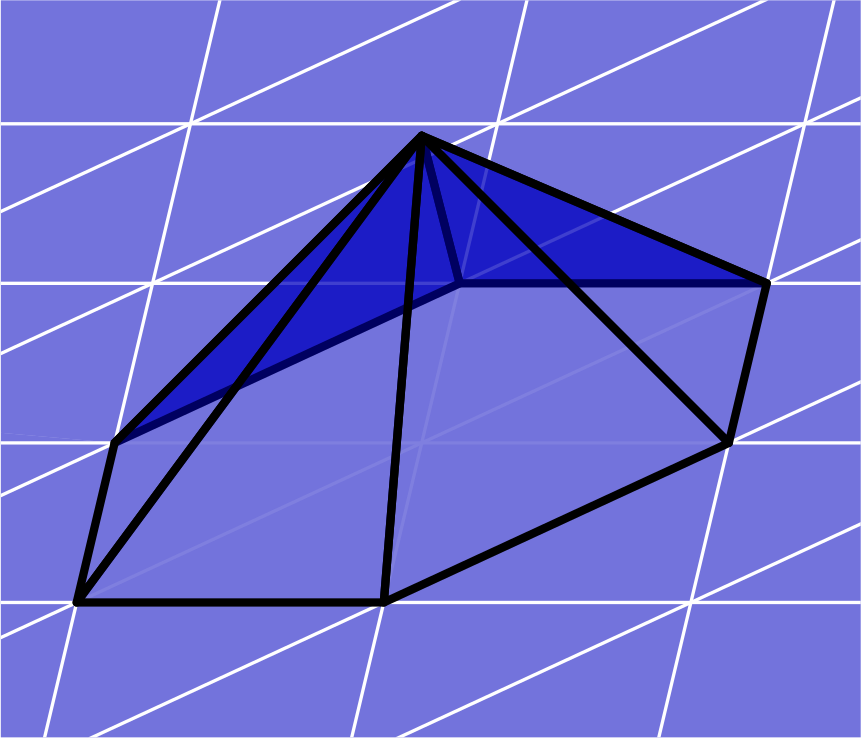
\includegraphics[width=0.6\textwidth]{../img/p1.png}

\footnotesize{Continuous polynomial order 1 basis function}\end{center}

This space can be created in Bempp with:

\begin{python}
space = bempp.api.function_space(grid, "P", 1)
\end{python}

The DOFs of an order 1 P space are at the three vertices of each cell.

\subsection{ Barycentric dual spaces}To define the barycentric dual space, we first create the barycentrically refined mesh by joining
each vertex of every triangle with the centre of the opposite side, as shown below.
\begin{center}
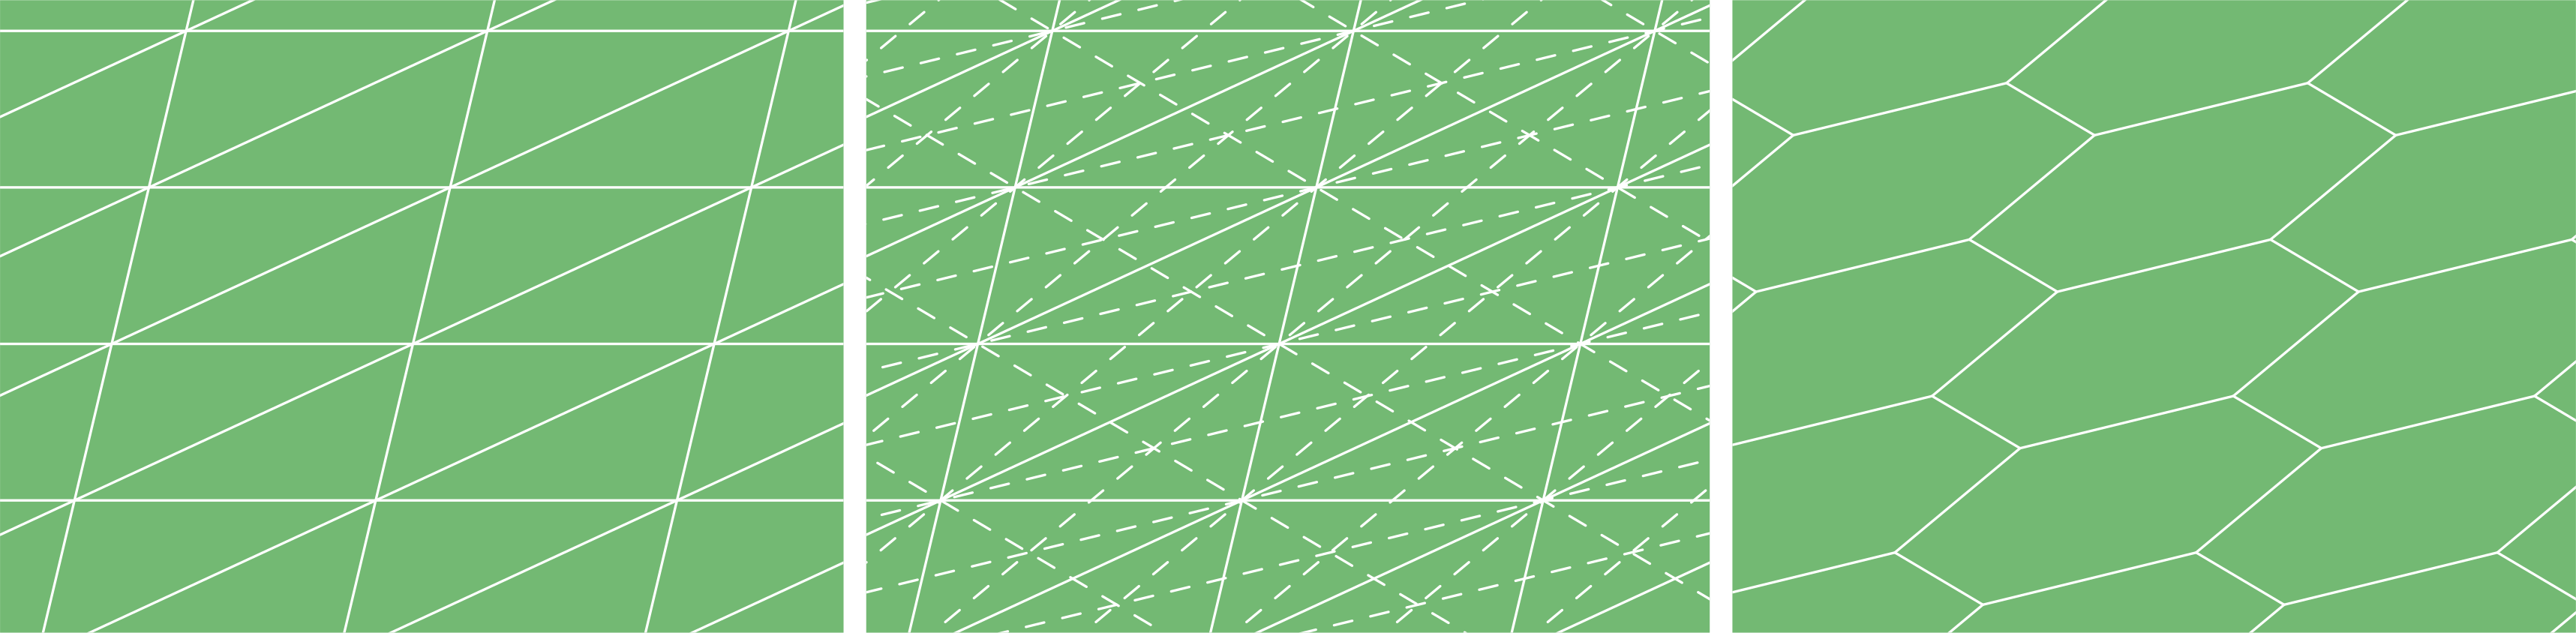
\includegraphics[width=0.6\textwidth]{../img/barycentric_mesh.png}

\footnotesize{Barycentrically refining a grid}\end{center}

The order 0 dual spaces are piecewise constant functions on the dual cells.
An example basis function of an order 0 DUAL space is shown below.
Order 0 DUAL spaces form a stable dual pairing with order 1 P spaces.
\begin{center}
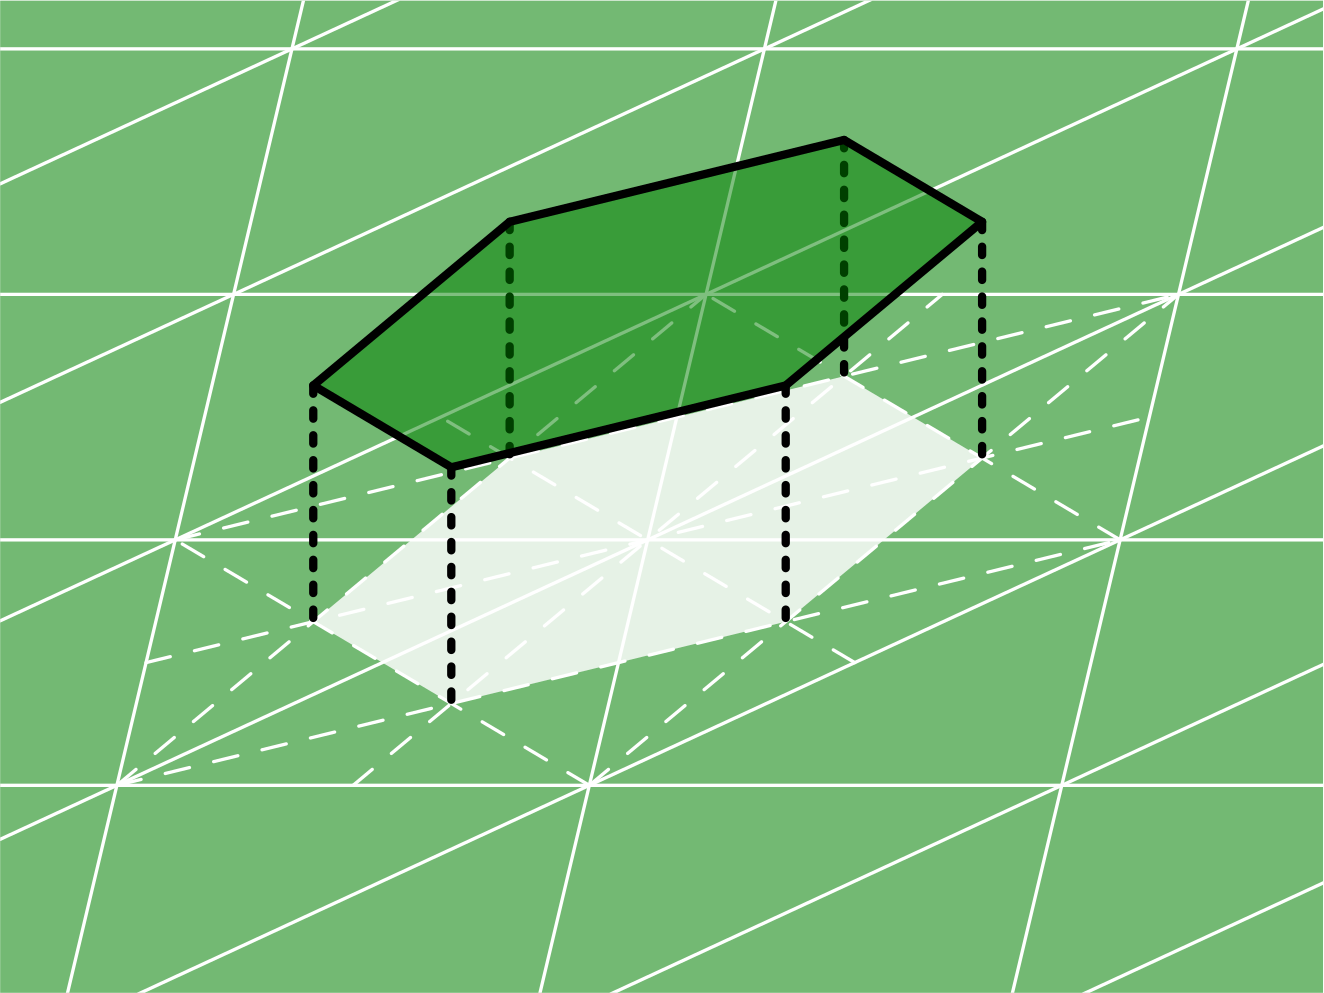
\includegraphics[width=0.6\textwidth]{../img/dual0.png}

\footnotesize{Dual order 0 basis function}\end{center}

The order 1 dual basis functions are linear combinations of piecewise linear
functions on the barycentric cells, and are defined in
\href{https://www.jstor.org/stable/40234460?seq=1}{\emph{A dual finite element complex on the barycentric refinement} (2007) by A. Buffa and S. Christiansen}.
An example basis function of an order 1 DUAL space is shown below.
Order 1 DUAL spaces form a stable dual pairing with order 0 DP spaces.
\begin{center}
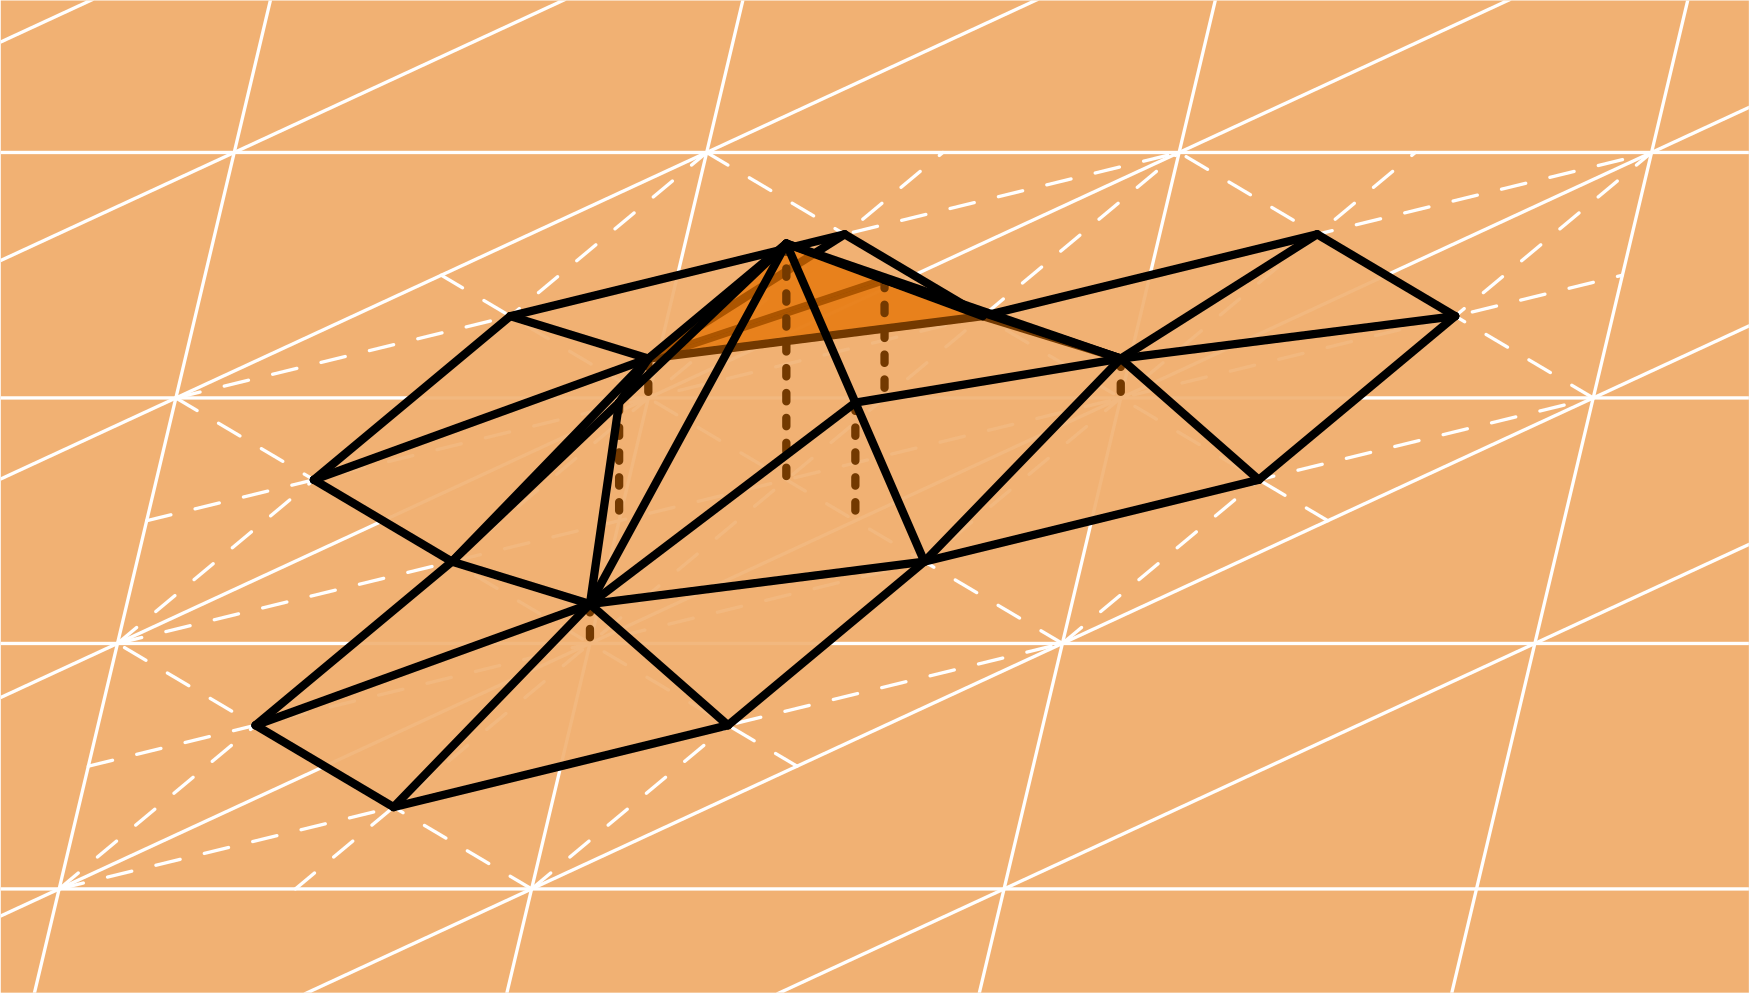
\includegraphics[width=0.6\textwidth]{../img/dual1.png}

\footnotesize{Dual order 1 basis function}\end{center}

These spaces can be created in Bempp with:

\begin{python}
space = bempp.api.function_space(grid, "DUAL", 0)
space = bempp.api.function_space(grid, "DUAL", 1)
\end{python}

The DOFs of an order 0 DUAL space are at the three vertices of each cell
(ie the midpoints of each barycentric dual cell).
The DOFs of an order 1 DUAL space are at the mispoints of each cell
(ie the vertices of each barycentric dual cell).


\section{Vector Function Spaces}


The following vector-valued spaces are supported in Bempp:

\begin{center}
\begin{tabular}{|l|l|l|}
\hline
Space Type & Order & Description\\
\hline
\verb@"RWG"@    & 0     & Rao--Wilson--Glisson Hdiv functions\\
\verb@"SNC"@    & 0     & Scaled N\'ed\'elec Hcurl functions\\
\verb@"BC"@     & 0     & Buffa--Christiansen Hdiv functions\\
\verb@"RBC"@    & 0     & Rotated Buffa--Christiansen Hcurl functions\\
\hline
\end{tabular}
\end{center}
When solving Maxwell's equations, the correct combination of Hdiv and Hcurl spaces must be used.

\subsection{ RWG and SNC spaces}RWG and SNC spaces are vector-valued spaces, whose values are tangential to the surface triangles.
Inside each cell, these spaces are linear combinations of the vectors
$\left(\begin{array}{c}1\\\\0\end{array}\right)$,
$\left(\begin{array}{c}0\\\\1\end{array}\right)$, and
$\left(\begin{array}{c}-y\\\\x\end{array}\right)$. Between cells, RWG functions are continuous normal
to the triangle's edges, while SNC spaces are continuous tangential to the triangle's edges.
Example RWG (left) and SNC (right) basis functions are shown below.

\begin{center}
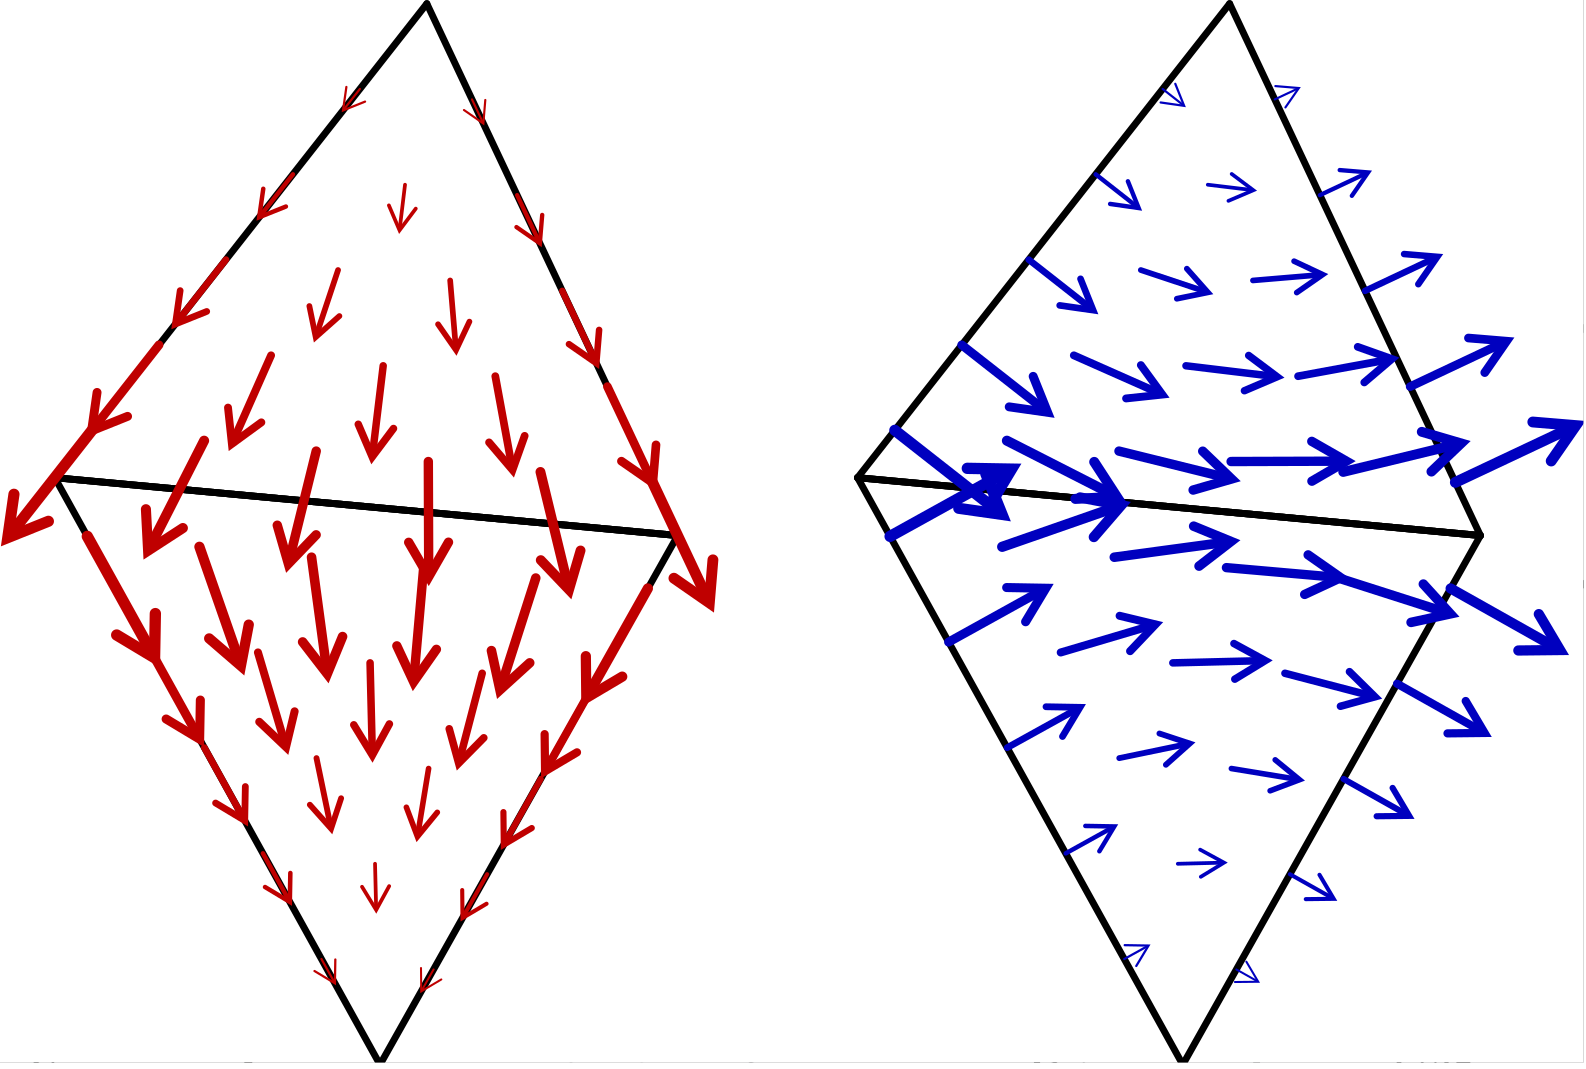
\includegraphics[width=0.6\textwidth]{../img/rwg_and_snc.png}

\footnotesize{An RWG and a SNC basis function}\end{center}

These spaces can be created in Bempp with:

\begin{python}
rwg_space = bempp.api.function_space(grid, "RWG", 0)
snc_space = bempp.api.function_space(grid, "SNC", 0)
\end{python}

The DOFs of RWG and SNC spaces are at the midpoints of the edges of each cell.

\subsection{ Barycentric dual spaces}Like the scalar DUAL spaces, BC and RBC spaces are defined on the barycentrically refined grid.
This grid is formed by joining
each vertex of every triangle with the centre of the opposite side, as shown below.
\begin{center}
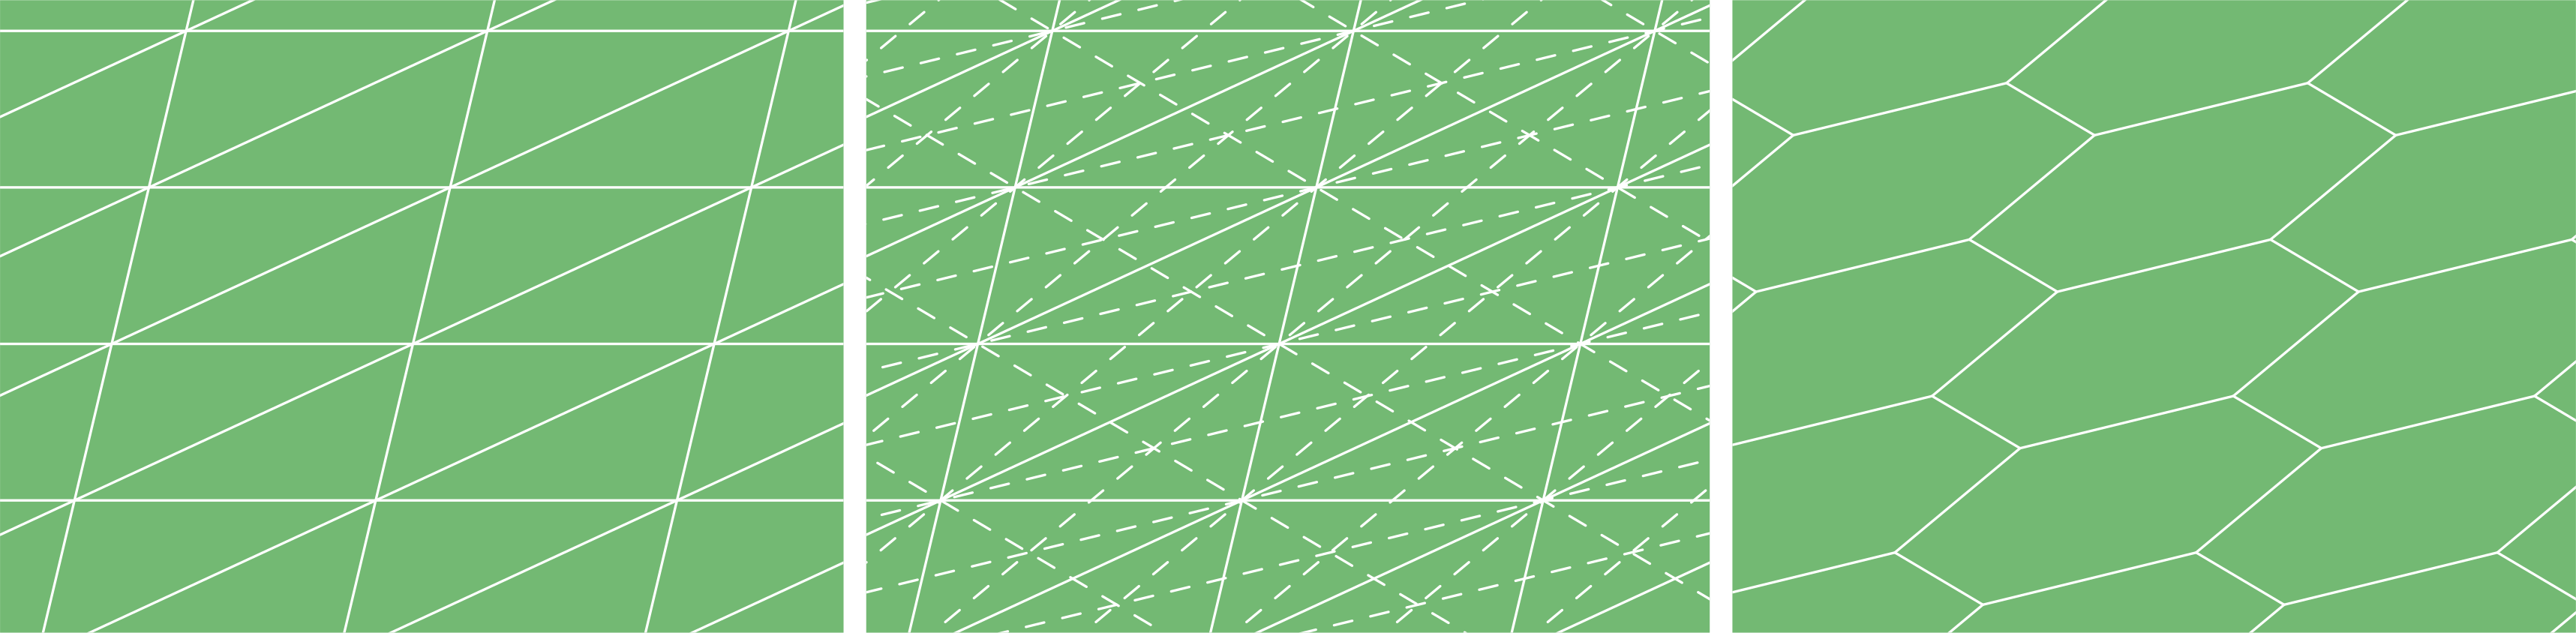
\includegraphics[width=0.6\textwidth]{../img/barycentric_mesh.png}

\footnotesize{Barycentrically refining a grid}\end{center}

BC and RBC spaces are combinations of RWG and SNC (repectively) spaces on the barycentric grid,
and are defined in
\href{https://www.jstor.org/stable/40234460?seq=1}{\emph{A dual finite element complex on the barycentric refinement} (2007) by A. Buffa and S. Christiansen}.
Example BC (left) and RBC (right) basis functions are shown below.

\begin{center}
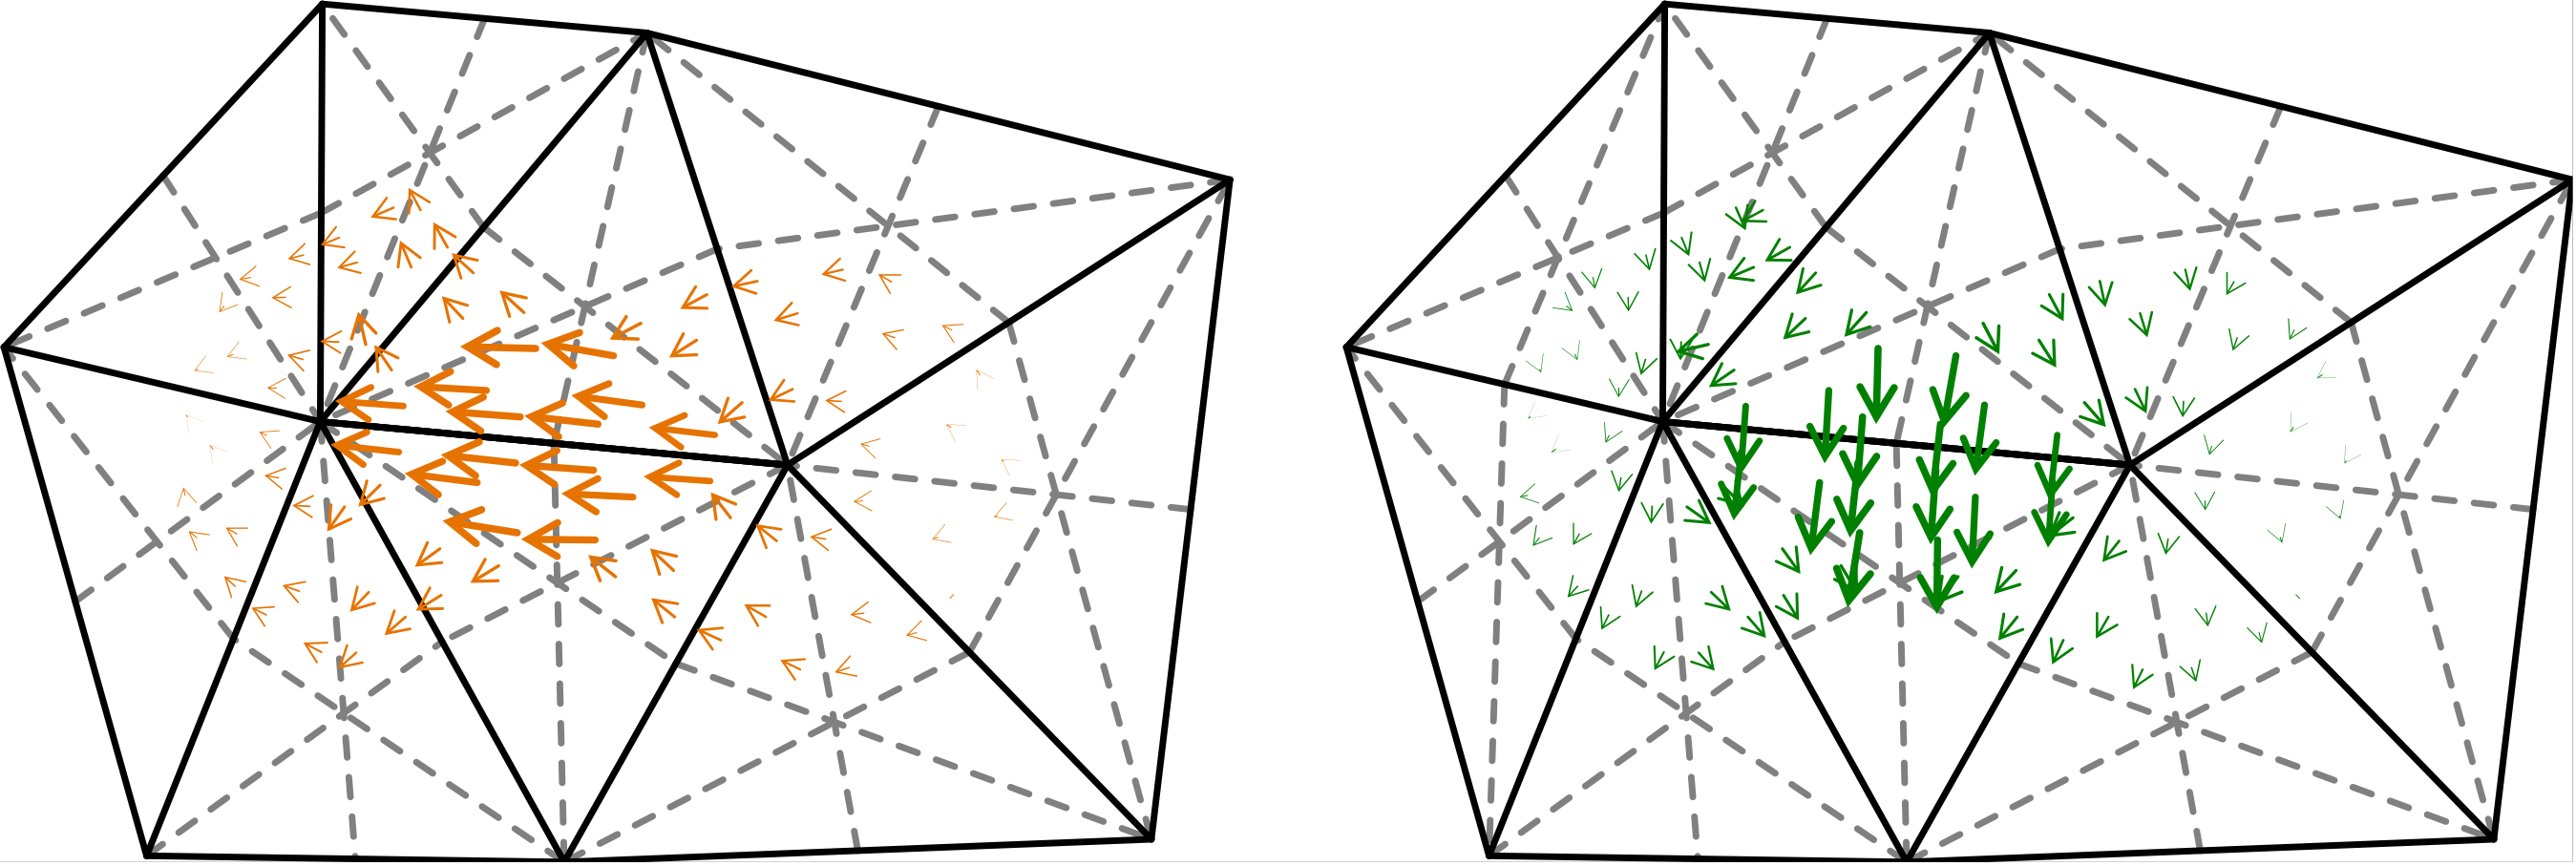
\includegraphics[width=0.6\textwidth]{../img/bc_and_rbc.png}

\footnotesize{Dual order 0 basis function}\end{center}

These spaces can be created in Bempp with:

\begin{python}
bc_space = bempp.api.function_space(grid, "BC", 0)
rbc_space = bempp.api.function_space(grid, "RBC", 0)
\end{python}

The DOFs of BC and RBC spaces are at the midpoints of the edges of each cell (or equivalently at
a point on the edges of the barycentric dual cells).


\section{Function Spaces on Segments}

Bempp can create spaces on segments of a grid as well as on the entire grid.
In order to do this, domain indices must be provided when \href{creating_grids.md}{creating the grid}.
Some built-in grids have domain indices: for example, the cube has six segments
for the faces (numbered 1 to 6).

To create a space on a segment, first create the grid:
\begin{python}
grid = bempp.api.shapes.cube()
\end{python}

A space on segments 1 and 2 of the grid can then be created using:
\begin{python}
space = bempp.api.function_space(grid, "DP", 0, segments=[1, 2])
\end{python}

\subsection{ Controlling segment spaces}There are two options that can be used to control the behaviour of a space on a segment:
\pyth{include_boundary_dofs} and \pyth{truncate_at_segment_edge}.

If \pyth{include_boundary_dofs} is set to \pyth{True}, DOF points on vertices and edges on the boundary.
By default, this is set to \pyth{False}. Setting this option to \pyth{True} is likely to make the
function space extend outside its segments, as part of the basis functions with DOFs on the
boundary will be outside the domain.

The option \pyth{truncate_at_segment_edge} can be used to truncate basis functions at the edge of the
segment, whenever a basis function will extend outside the segments. By default, this is \pyth{False}.
Setting this option to \pyth{True} will cause the function space to be discontinuous at the edge
of the segment.


\chapter{Grid functions}


In Bempp, data on a given grid is represented as a grid function object.
A grid function consists of a set of basis function coefficients and a corresponding \href{function_spaces.md}{function space}.


\section{ Initialising with a Python callable}Grid functions can be created from Python callables.

\begin{python}
@bempp.api.complex_callable
def fun(x, normal, domain_index, result):
    result[0] = np.exp(1j * x[0])
\end{python}

The first argument \pyth{x} is the coordinates of an evaluation point.
The second argument \pyth{normal} is the normal direction at the evaluation point.
The third one is the \pyth{domain_index}: this corresponds to the physical id in Gmsh and can be used to assign different boundary data to different parts of the grid.
The last argument \pyth{result} is the variable that stores the value of the callable.
It is a Numpy array with as many components as the basis functions of the underlying space have.

A Python callable that you want to use to build a grid function should always have these four inputs.
An optional fifth input may be used to pass parameters into the function.

In order for Bempp to assemble a grid function with coefficients of the correct data type,
these callables must be decorated with either \pyth{@bempp.api.real_callable} or
\pyth{@bempp.api.real_callable}.

The projection of this callable into a Bempp space can be created with:
\begin{python}
grid_fun = bempp.api.GridFunction(space, fun=fun)
\end{python}

\subsection{ Disabling just-in-time compilation}By default, Bempp with use Numba just-in-time compilation when creating grid functions from callables.
In some cases, this compilation is not possible and should be disabled. This can be
done by passing \pyth{jit=False} into the decorator:

\begin{python}
@bempp.api.complex_callable(jit=False)
def fun(x, normal, domain_index, result):
    result[0] = np.exp(1j * x[0])

grid_fun = bempp.api.GridFunction(space, fun=fun)
\end{python}

The construction of this grid function will be slower as it is not sped up by Numba.

\section{ Initialising with coefficients or projections}Instead of a callable, we can initialise a grid function from a vector of
coefficients or a vector of projections.
This can be done as follows.

\begin{python}
c = np.array([...])  # These are the coefficients
grid_fun = GridFunction(space, coefficients=c)

p = np.array([...])  # These are the projections
grid_fun = GridFunction(space, projections=p, dual_space=dual)
\end{python}

The argument \pyth{dual_space} gives the space with which the projection coefficients were computed.
The parameter is optional and if it is not given then \pyth{space == dual_space} is assumed.

\section{ Coefficients and projections}The functions in a discrete function space are represented as a linear combination of some basis
functions. The coefficients of a grid function are the scalars which each basis function
is multiplied by in this combination. The coefficients of a grid function can be obtained using:

\begin{python}
grid_fun.coefficients
\end{python}

The projections of a grid function are calculated by applying a discrete mass matrix to the
coefficients. The mass matrix will be between the grid function's space and a dual space
provided to the \pyth{projections} call. These can be obtained using:

\begin{python}
grid_fun.projections(dual_space)
\end{python}

In some situations, for example when the space and the dual are RWG and SNC spaces, the mass matrix
for projections may be numerically singular. In these cases, the coefficients of a grid function
that has been initialised using projections cannot be accurately calculated. Bempp, however, can
still use these grid functions by only querying the projections.

\section{ Plotting and exporting grid functions}To export a grid function, we can use the \pyth{export} command:

\begin{python}
bempp.api.export('grid_function.msh', grid_function=grid_fun)
\end{python}

This commands export the object \pyth{grid_fun} as Gmsh file with the
name \pyth{grid_function.msh}.

In order to plot a grid function, we can simply use the command:

\begin{python}
grid_fun.plot()
\end{python}

By default, this will plot using Gmsh (or plotly if you are inside a Jupyter notebook).
The following command can be used to change the plotting backend.

\begin{python}
bempp.api.PLOT_BACKEND = "gmsh"
bempp.api.PLOT_BACKEND = "paraview"
\end{python}

This requires Gmsh or Paraview to be available in the system path.


\chapter{Boundary Operators}


Boundary integral formulations of problems are commonly written using boundary integral operators.
In this section of the Bempp Handbook, we look at how these operators can be defined and
assembled using Bempp.

\section{ Domains, ranges, and duals}When creating an operator in Bempp, three spaces are provided: the domain, the range, and the
dual to the range (given as inputs in that order). The domain and dual spaces are used to
calculate the weak form of the operator. The range is used by the
\href{operator_algebra.md}{operator algebra} to correctly assemble product of operators.


\section{Sparse Boundary Operators}

Discretising the identity operator leads to a matrix $M=(m_{ij})$, defined by
\[m_{ij}=\int_\Gamma\phi_j\cdot\overline{\psi_i},\]
where $\phi_j$ and $\psi_i$ are the basis functions of the domain and dual spaces respectively.
As this integral will only be non-zero when the basis functions overlap, the resulting
matrix will be sparse.

The identity operator can be created in Bempp using:
\begin{python}
ident = bempp.api.operators.boundary.sparse(domain, range_, dual)
\end{python}

A \pyth{SparseDiscreteBoundaryOperator} can be obtained using:
\begin{python}
mat = ident.weak_form()
\end{python}
This matrix is commonly called the mass matrix between the domain and dual spaces.

If desiried, a SciPy CSR matrix can be obtained from this discrete boundary operator with:
\begin{python}
mat.A
\end{python}


\section{Boundary Operators for Laplace's Equation}

For Laplace's equation, there are four boundary operators that are used, as given in the table
below.

\begin{center}
\begin{tabular}{|l|l|l|}
\hline
Operator             & Symbol        & Matrix entries\\
\hline
Single layer         & $\mathsf{V}$  & $\displaystyle m_{ij}=\int_{\Gamma}\int_{\Gamma}G(\mathbf{x},\mathbf{y})\phi_j(\mathbf{y})\psi_i(\mathbf{x})\,\mathrm{d}\mathbf{y}\,\mathrm{d}\mathbf{x}$\\
Double layer         & $\mathsf{K}$  & $\displaystyle m_{ij}=\int_{\Gamma}\int_{\Gamma}\frac{\partial G(\mathbf{x},\mathbf{y})}{\partial\mathbf{\nu}_{\mathbf{y}}}\phi_j(\mathbf{y})\psi_i(\mathbf{x})\,\mathrm{d}\mathbf{y}\,\mathrm{d}\mathbf{x}$\\
Adjoint double layer & $\mathsf{K}'$ & $\displaystyle m_{ij}=\int_{\Gamma}\int_{\Gamma}\frac{\partial G(\mathbf{x},\mathbf{y})}{\partial\mathbf{\nu}_{\mathbf{x}}}\phi_j(\mathbf{y})\psi_i(\mathbf{x})\,\mathrm{d}\mathbf{y}\,\mathrm{d}\mathbf{x}$\\
Hypersingular        & $\mathsf{W}$  & $\displaystyle m_{ij}=\int_{\Gamma}\int_{\Gamma}\frac{\partial^2 G(\mathbf{x},\mathbf{y})}{\partial\mathbf{\nu}_{\mathbf{y}}\partial\mathbf{\nu}_{\mathbf{x}}}\phi_j(\mathbf{y})\psi_i(\mathbf{x})\,\mathrm{d}\mathbf{y}\,\mathrm{d}\mathbf{x}$\\
\hline
\end{tabular}
\end{center}
In each case,  $\phi_j$ and $\psi_i$ are the basis functions of the domain and dual spaces (respectively),
and $G(\mathbf{x},\mathbf{y})$ is the Green's function for Laplace's equation.
The Green's function will have a singularity when $\mathbf{x}=\mathbf{y}$, so internally Bempp will
use appropriate singular quadrature rules to handle this.

These operators can be initialised in Bempp using:
\begin{python}
from bempp.api.operators.boundary import laplace
single = laplace.single_layer(domain, range_, dual)
double = laplace.double_layer(domain, range_, dual)
adjoint_d = laplace.adjoint_double_layer(domain, range_, dual)
hypersingular = laplace.hypersingular(domain, range_, dual)
\end{python}
The spaces passed into each operator should be appropriately chosen
\href{scalar_function_spaces.md}{scalar function spaces}.

A keyword argument \pyth{assembler} may be passed into each constructor to change the assembler
used to assemble the operator. For example, the single layer operator will be discretised using
the fast multipole method (FMM) if it is initialised with:
\begin{python}
single = laplace.single_layer(domain, range_, dual, assembler="fmm")
\end{python}

When using dense assembly, the keyword argument \pyth{device_interface} can be used to switch
between assembly using OpenCL and Numba:
\begin{python}
single = laplace.single_layer(
    domain, range_, dual, wavenumber, assembler="dense",
    device_interface="numba"
    )
single = laplace.single_layer(
    domain, range_, dual, wavenumber, assembler="dense",
    device_interface="opencl"
    )
\end{python}

The matrix discretisation of an operator can be obtained using, for example:

\begin{python}
single.weak_form()
\end{python}

The strong form discretisation of an operator can be obtained using:
\begin{python}
single.strong_form()
\end{python}
The interpretation of the strong form is discussed in the \href{operator_algebra.md}{operator algebra}
section.


\section{Boundary Operators for the Helmholtz Equation}

For the Helmholtz equation, there are four boundary operators that are used, as given in the table
below.

\begin{center}
\begin{tabular}{|l|l|l|}
\hline
Operator             & Symbol        & Matrix entries\\
\hline
Single layer         & $\mathsf{V}$  & $\displaystyle m_{ij}=\int_{\Gamma}\int_{\Gamma}G_k(\mathbf{x},\mathbf{y})\phi_j(\mathbf{y})\psi_i(\mathbf{x})\,\mathrm{d}\mathbf{y}\,\mathrm{d}\mathbf{x}$\\
Double layer         & $\mathsf{K}$  & $\displaystyle m_{ij}=\int_{\Gamma}\int_{\Gamma}\frac{\partial G_k(\mathbf{x},\mathbf{y})}{\partial\mathbf{\nu}_{\mathbf{y}}}\phi_j(\mathbf{y})\psi_i(\mathbf{x})\,\mathrm{d}\mathbf{y}\,\mathrm{d}\mathbf{x}$\\
Adjoint double layer & $\mathsf{K}'$ & $\displaystyle m_{ij}=\int_{\Gamma}\int_{\Gamma}\frac{\partial G_k(\mathbf{x},\mathbf{y})}{\partial\mathbf{\nu}_{\mathbf{x}}}\phi_j(\mathbf{y})\psi_i(\mathbf{x})\,\mathrm{d}\mathbf{y}\,\mathrm{d}\mathbf{x}$\\
Hypersingular        & $\mathsf{W}$  & $\displaystyle m_{ij}=\int_{\Gamma}\int_{\Gamma}\frac{\partial^2 G_k(\mathbf{x},\mathbf{y})}{\partial\mathbf{\nu}_{\mathbf{y}}\partial\mathbf{\nu}_{\mathbf{x}}}\phi_j(\mathbf{y})\psi_i(\mathbf{x})\,\mathrm{d}\mathbf{y}\,\mathrm{d}\mathbf{x}$\\
\hline
\end{tabular}
\end{center}
In each case,  $\phi_j$ and $\psi_i$ are the basis functions of the domain and dual spaces (respectively),
and $G_k(\mathbf{x},\mathbf{y})$ is the Green's function for the Helmholtz equation with
wavenumber $k$.
The Green's function will have a singularity when $\mathbf{x}=\mathbf{y}$, so internally Bempp will
use appropriate singular quadrature rules to handle this.

These operators can be initialised in Bempp using:
\begin{python}
from bempp.api.operators.boundary import helmholtz
single = helmholtz.single_layer(domain, range_, dual, wavenumber)
double = helmholtz.double_layer(domain, range_, dual, wavenumber)
adjoint_d = helmholtz.adjoint_double_layer(domain, range_, dual, wavenumber)
hypersingular = helmholtz.hypersingular(domain, range_, dual, wavenumber)
\end{python}
The spaces passed into each operator should be appropriately chosen
\href{scalar_function_spaces.md}{scalar function spaces}.

A keyword argument \pyth{assembler} may be passed into each constructor to change the assembler
used to assemble the operator. For example, the single layer operator will be discretised using
the fast multipole method (FMM) if it is initialised with:
\begin{python}
single = helmholtz.single_layer(
    domain, range_, dual, wavenumber, assembler="fmm")
\end{python}

When using dense assembly, the keyword argument \pyth{device_interface} can be used to switch
between assembly using OpenCL and Numba:
\begin{python}
single = helmholtz.single_layer(
    domain, range_, dual, wavenumber, assembler="dense",
    device_interface="numba"
    )
single = helmholtz.single_layer(
    domain, range_, dual, wavenumber, assembler="dense",
    device_interface="opencl"
    )
\end{python}

The matrix discretisation of an operator can be obtained using, for example:

\begin{python}
single.weak_form()
\end{python}

The strong form discretisation of an operator can be obtained using:
\begin{python}
single.strong_form()
\end{python}
The interpretation of the strong form is discussed in the \href{operator_algebra.md}{operator algebra}
section.


\section{Boundary Operators for the Modified Helmholtz Equation}

For the modified Helmholtz equation, there are four boundary operators that are used, as given in the table
below.

\begin{center}
\begin{tabular}{|l|l|l|}
\hline
Operator             & Symbol        & Matrix entries\\
\hline
Single layer         & $\mathsf{V}$  & $\displaystyle m_{ij}=\int_{\Gamma}\int_{\Gamma}G_\omega(\mathbf{x},\mathbf{y})\phi_j(\mathbf{y})\psi_i(\mathbf{x})\,\mathrm{d}\mathbf{y}\,\mathrm{d}\mathbf{x}$\\
Double layer         & $\mathsf{K}$  & $\displaystyle m_{ij}=\int_{\Gamma}\int_{\Gamma}\frac{\partial G_\omega(\mathbf{x},\mathbf{y})}{\partial\mathbf{\nu}_{\mathbf{y}}}\phi_j(\mathbf{y})\psi_i(\mathbf{x})\,\mathrm{d}\mathbf{y}\,\mathrm{d}\mathbf{x}$\\
Adjoint double layer & $\mathsf{K}'$ & $\displaystyle m_{ij}=\int_{\Gamma}\int_{\Gamma}\frac{\partial G_\omega(\mathbf{x},\mathbf{y})}{\partial\mathbf{\nu}_{\mathbf{x}}}\phi_j(\mathbf{y})\psi_i(\mathbf{x})\,\mathrm{d}\mathbf{y}\,\mathrm{d}\mathbf{x}$\\
Hypersingular        & $\mathsf{W}$  & $\displaystyle m_{ij}=\int_{\Gamma}\int_{\Gamma}\frac{\partial^2 G_\omega(\mathbf{x},\mathbf{y})}{\partial\mathbf{\nu}_{\mathbf{y}}\partial\mathbf{\nu}_{\mathbf{x}}}\phi_j(\mathbf{y})\psi_i(\mathbf{x})\,\mathrm{d}\mathbf{y}\,\mathrm{d}\mathbf{x}$\\
\hline
\end{tabular}
\end{center}
In each case,  $\phi_j$ and $\psi_i$ are the basis functions of the domain and dual spaces (respectively),
and $G_\omega(\mathbf{x},\mathbf{y})$ is the Green's function for the modified Helmholtz equation with
frequency $\omega$.
The Green's function will have a singularity when $\mathbf{x}=\mathbf{y}$, so internally Bempp will
use appropriate singular quadrature rules to handle this.

These operators can be initialised in Bempp using:
\begin{python}
from bempp.api.operators.boundary import modified_helmholtz
single = modified_helmholtz.single_layer(domain, range_, dual, omega)
double = modified_helmholtz.double_layer(domain, range_, dual, omega)
adjoint_d = modified_helmholtz.adjoint_double_layer(domain, range_, dual, omega)
hypersingular = modified_helmholtz.hypersingular(domain, range_, dual, omega)
\end{python}
The spaces passed into each operator should be appropriately chosen
\href{scalar_function_spaces.md}{scalar function spaces}.

A keyword argument \pyth{assembler} may be passed into each constructor to change the assembler
used to assemble the operator. For example, the single layer operator will be discretised using
the fast multipole method (FMM) if it is initialised with:
\begin{python}
single = modified_helmholtz.single_layer(
    domain, range_, dual, omega, assembler="fmm")
\end{python}

When using dense assembly, the keyword argument \pyth{device_interface} can be used to switch
between assembly using OpenCL and Numba:
\begin{python}
single = modified_helmholtz.single_layer(
    domain, range_, dual, wavenumber, assembler="dense",
    device_interface="numba"
    )
single = modified_helmholtz.single_layer(
    domain, range_, dual, wavenumber, assembler="dense",
    device_interface="opencl"
    )
\end{python}

The matrix discretisation of an operator can be obtained using, for example:

\begin{python}
single.weak_form()
\end{python}

The strong form discretisation of an operator can be obtained using:
\begin{python}
single.strong_form()
\end{python}
The interpretation of the strong form is discussed in the \href{operator_algebra.md}{operator algebra}
section.


\section{Boundary Operators for Maxwell's Equations}

For Maxwell's equations, there are two boundary operators that are used, as given in the table
below.

\begin{center}
\begin{tabular}{|l|l|l|}
\hline
Operator             & Symbol       & Matrix entries\\
\hline
Electric field       & $\mathsf{E}$ & $\displaystyle m_{ij}=-\mathrm{i}k\int_\Gamma\int_\Gamma G_k(\mathbf{x},\mathbf{y})\mathbf{\phi}_j(\mathbf{y})\cdot\mathbf{\psi}_i(\mathbf{x})\,\mathrm{d}\mathbf{y}\,\mathrm{d}\mathbf{x}-\frac{1}{\mathrm{i}k}\int_\Gamma\int_\Gamma G_k(\mathrm{x},\mathrm{y})\nabla_\Gamma\mathbf{\phi}_j(\mathbf{y})\nabla_\Gamma\mathbf{\psi}_i(\mathbf{x})\,\mathrm{d}\mathbf{y}\,\mathrm{d}\mathbf{x})$\\
Magnetic field       & $\mathsf{H}$ & $\displaystyle m_{ij}=-\int_\Gamma\int_\Gamma\nabla_\mathbf{x}G_k(\mathbf{x},\mathbf{y})\cdot(\mathbf{\psi}_j(\mathbf{y})\times\mathbf{\psi}_i(\mathbf{x}))\,\mathrm{d}\mathbf{y}\,\mathrm{d}\mathbf{x})$\\
\hline
\end{tabular}
\end{center}

In each case,  $\phi_j$ and $\psi_i$ are the basis functions of the domain and dual spaces (respectively),
and $G_k(\mathbf{x},\mathbf{y})$ is the Green's function for the Helmholtz equation with
wavenumber $k$.
The Green's function will have a singularity when $\mathbf{x}=\mathbf{y}$, so internally Bempp will
use appropriate singular quadrature rules to handle this.

These operators can be initialised in Bempp using:
\begin{python}
from bempp.api.operators.boundary import maxwell
electric = maxwell.electric_field(domain, range_, dual, wavenumber)
magnetic = maxwell.magnetic_field(domain, range_, dual, wavenumber)
\end{python}
The spaces passed into each operator should be appropriately chosen
\href{vector_function_spaces.md}{vector function spaces}: the domain and range spaces
should both be Hdiv spaces, while the dual space should be a Hcurl space.

A keyword argument \pyth{assembler} may be passed into each constructor to change the assembler
used to assemble the operator. For example, the electric field operator will be discretised using
the fast multipole method (FMM) if it is initialised with:
\begin{python}
electric = maxwell.electric_field(
    domain, range_, dual, wavenumber, assembler="fmm")
\end{python}

When using dense assembly, the keyword argument \pyth{device_interface} can be used to switch
between assembly using OpenCL and Numba:
\begin{python}
electric = maxwell.electric_field(
    domain, range_, dual, wavenumber, assembler="dense",
    device_interface="numba"
    )
electric = maxwell.electric_field(
    domain, range_, dual, wavenumber, assembler="dense",
    device_interface="opencl"
    )
\end{python}

The matrix discretisation of an operator can be obtained using, for example:

\begin{python}
electric.weak_form()
\end{python}

The strong form discretisation of an operator can be obtained using:
\begin{python}
electric.strong_form()
\end{python}
The interpretation of the strong form is discussed in the \href{operator_algebra.md}{operator algebra}
section. For Maxwell's equations, care must be taken to use space for the range and dual spaces
that form a stable dual pairing (see the \href{vector_function_spaces.md}{vector function spaces}
section) in order to be able to correctly obtain the strong form of an operator.


\section{Operator Algebra}

In many boundary element method applications, a discretisation of the product of two operators
is required.

Let $\mathsf{A}$ and $\mathsf{B}$ be two operators with discretisations $A_h$ and $B_h$.
A discretisation of the product $\mathsf{A}\mathsf{B}$ is given by $A_hM^{-1}B_h$,
where $M$ is the mass matrix between the range and dual of the operator $\mathsf{B}$.

In Bempp, the discrete product of two operators can be formed using:
\begin{python}
op1 = bempp.api.operators.boundary...
op2 = bempp.api.operators.boundary...
product = op1 * op2
\end{python}
If \pyth{product.weak_form()} is called, Bempp will internally use its knowledge of the range space
of \pyth{op2} to correctly from the discretisation of this product.

Calling the \pyth{strong_form} of an operator $\mathsf{B}$ will return the product
$M^{-1}B_h$. Calling \pyth{product.weak_form()} is equivalent to calculating
\pyth{op1.weak_form() * op2.strong_form()}. Using the strong form of operators can in general
be useful, as the discretisation obtained corresponds to a mass matrix preconditioned
version of the relevant formulation.


\chapter{Linear Solvers}


Once you have assembled the relevant operators, and have created a grid function containing
the relevant right-hand-side data, you will need to solve your linear system.


\section{Direct Solvers}


Direct solvers compute the solution of a linear system by (usually indirectly) computing the
inverse of the matrix.

SciPy's direct LU solver is wrapped in the function \pyth{bempp.api.linalg.lu}. This can be used with:
\begin{python}
solution = bempp.api.linalg.lu(operator, grid_fun)
\end{python}

Direct solvers should only be used if the operator has been assembled in dense mode.


\section{Iterative Solvers}


Iterative solvers solve a linear system iteratively: steps are repeated to achieve better
approximations of the solution. For well-condtioned matrices, iterative solvers can achieve
fast convergence, so very good approximations of the solution can be achieved in just a few
iterations.

SciPy's CG and GMRes iterative solvers are wrapped in the \pyth{bempp.api.linalg} submodule. These
can be used with:

\begin{python}
solution, info = bempp.api.linalg.cg(operator, grid_fun)
solution, info = bempp.api.linalg.gmres(opreator, grid_fun)
\end{python}

These solvers take a number of optional arguments:

\begin{center}
\begin{tabular}{|l|l|l|}
\hline
Argument  & Description & Default\\
\hline
\verb@tol@     & The tolerance the solver should aim for & \verb@1e-5@\\
\verb@maxiter@ & The maximum number of iterations & No maximum\\
\verb@use_strong_form@ & If \verb@True@, the strong form of the operator will be used. If \verb@False@, the weak form is used. & \verb@False@\\
\verb@return_residuals@ & If \verb@True@ the residuals will be returned as well as the solution and info & \verb@False@\\
\verb@return_iteration_count@ & If \verb@True@ the iteration count will be returned as well as the solution and info & \verb@False@\\
\hline
\end{tabular}
\end{center}
By default, Bempp will use the weak form discretisation of the operator and the coefficients
of the grid function when using an iterative solver.
If \pyth{use_strong_form} is set to \pyth{True}, Bempp will use the strong form discretisation of the operator
and the projections of the grid function onto the range of the operator. This is equivalent
to applying a mass matrix preconditioner to the problem and often leads to a lower iteration count.


\chapter{Potential Operators}


Once the solution of a boundary integral formulation has been approximated, potential
operators can be used to compute point evaluations of the solution inside the domain.


\section{Potential Operators for Laplace's Equation}

For Laplace's equation, there are two potential operators that are used, as given in the table
below.

\begin{center}
\begin{tabular}{|l|l|}
\hline
Operator             & Definition\\
\hline
Single layer         & $\displaystyle (\mathcal{V}\mu)(\mathbf{x}) := \int_{\Gamma} G(\mathbf{x},\mathbf{y}) \mu(\mathbf{y})\,\mathrm{d}\mathbf{y}$\\
Double layer         & $\displaystyle (\mathcal{K}v)(\mathbf{x}) := \int_{\Gamma} \frac{\partial G(\mathbf{x},\mathbf{y})}{\partial\mathbf{\nu}_{\mathbf{y}}} v(\mathbf{y})\,\mathrm{d}\mathbf{y}$\\
\hline
\end{tabular}
\end{center}

In each case, $G(\mathbf{x},\mathbf{y})$ is the Green's function for Laplace's equation.

To assemble potential operators in Bempp, the desired evaluation points must first be defined.
For example, the following snippet creates a grid of 2500 points in the $x$$y$-plane with
$x$ and $y$ between -3 and 3.

\begin{python}
plot_grid = np.mgrid[-3:3:50j, -3:3:50j]
points = np.vstack((plot_grid[0].ravel(),
                    plot_grid[1].ravel(),
                    np.zeros(plot_grid[0].size)))
\end{python}

Potential operators can thenbe initialised in Bempp using:
\begin{python}
from bempp.api.operators.potential import laplace
single = laplace.single_layer(domain, points)
double = laplace.double_layer(domain, points)
\end{python}

These can be applied to a grid function with:
\begin{python}
single.evaluate(solution)
double.evaluate(solution)
\end{python}

As with \href{laplace_boundary_operators.md}{boundary operators}, \pyth{assembler} and \pyth{device_interface}
keyword arguments can be used to control the assembly type used for potential operators.


\section{Potential Operators for the Helmholtz Equation}

For the Helmholtz equation, there are two potential operators that are used, as given in the table
below.

\begin{center}
\begin{tabular}{|l|l|}
\hline
Operator             & Definition\\
\hline
Single layer         & $\displaystyle (\mathcal{V}\mu)(\mathbf{x}) := \int_{\Gamma} G_k(\mathbf{x},\mathbf{y}) \mu(\mathbf{y})\,\mathrm{d}\mathbf{y}$\\
Double layer         & $\displaystyle (\mathcal{K}v)(\mathbf{x}) := \int_{\Gamma} \frac{\partial G_k(\mathbf{x},\mathbf{y})}{\partial\mathbf{\nu}_{\mathbf{y}}} v(\mathbf{y})\,\mathrm{d}\mathbf{y}$\\
\hline
\end{tabular}
\end{center}

In each case, $G_k(\mathbf{x},\mathbf{y})$ is the Green's function for the Helmholtz equation
with wavenumber $k$.

To assemble potential operators in Bempp, the desired evaluation points must first be defined.
For example, the following snippet creates a grid of 2500 points in the $x$$y$-plane with
$x$ and $y$ between -3 and 3.

\begin{python}
plot_grid = np.mgrid[-3:3:50j, -3:3:50j]
points = np.vstack((plot_grid[0].ravel(),
                    plot_grid[1].ravel(),
                    np.zeros(plot_grid[0].size)))
\end{python}

Potential operators can thenbe initialised in Bempp using:
\begin{python}
from bempp.api.operators.potential import helmholtz
single = helmholtz.single_layer(domain, points, wavenumber)
double = helmholtz.double_layer(domain, points, wavenumber)
\end{python}

These can be applied to a grid function with:
\begin{python}
single.evaluate(solution)
double.evaluate(solution)
\end{python}

As with \href{helmholtz_boundary_operators.md}{boundary operators}, \pyth{assembler} and \pyth{device_interface}
keyword arguments can be used to control the assembly type used for potential operators.


\section{Potential Operators for the modified Helmholtz Equation}

For the modified Helmholtz equation, there are two potential operators that are used, as given in the table
below.

\begin{center}
\begin{tabular}{|l|l|}
\hline
Operator             & Definition\\
\hline
Single layer         & $\displaystyle (\mathcal{V}\mu)(\mathbf{x}) := \int_{\Gamma} G_\omega(\mathbf{x},\mathbf{y}) \mu(\mathbf{y})\,\mathrm{d}\mathbf{y}$\\
Double layer         & $\displaystyle (\mathcal{K}v)(\mathbf{x}) := \int_{\Gamma} \frac{\partial G_\omega(\mathbf{x},\mathbf{y})}{\partial\mathbf{\nu}_{\mathbf{y}}} v(\mathbf{y})\,\mathrm{d}\mathbf{y}$\\
\hline
\end{tabular}
\end{center}

In each case, $G_\omega(\mathbf{x},\mathbf{y})$ is the Green's function for the modified Helmholtz equation
with frequency $\omega$.

To assemble potential operators in Bempp, the desired evaluation points must first be defined.
For example, the following snippet creates a grid of 2500 points in the $x$$y$-plane with
$x$ and $y$ between -3 and 3.

\begin{python}
plot_grid = np.mgrid[-3:3:50j, -3:3:50j]
points = np.vstack((plot_grid[0].ravel(),
                    plot_grid[1].ravel(),
                    np.zeros(plot_grid[0].size)))
\end{python}

Potential operators can thenbe initialised in Bempp using:
\begin{python}
from bempp.api.operators.potential import modified_helmholtz
single = modified_helmholtz.single_layer(domain, points, omega)
double = modified_helmholtz.double_layer(domain, points, omega)
\end{python}

These can be applied to a grid function with:
\begin{python}
single.evaluate(solution)
double.evaluate(solution)
\end{python}

As with \href{modified_helmholtz_boundary_operators.md}{boundary operators}, \pyth{assembler} and \pyth{device_interface}
keyword arguments can be used to control the assembly type used for potential operators.


\section{Potential Operators for Maxwell's Equations}

For Maxwell's equations, there are two potential operators that are used, as given in the table
below.

\begin{center}
\begin{tabular}{|l|l|}
\hline
Operator       & Definition\\
\hline
Electric field & $\displaystyle (\mathcal{E}(\mathbf{p}))(\mathbf{x})=\mathrm{i} k\int_\Gamma\mathbf{p}(\mathbf{y})G_k(\mathbf{x},\mathbf{y})\,\mathrm{d}\mathbf{y}-\frac1{\mathrm{i} k}\nabla_{\mathbf{x}}\int_\Gamma\nabla_{\Gamma}\cdot\mathbf{p}(\mathbf{y})G_k(\mathbf{x},\mathbf{y})\,\mathrm{d}\mathbf{y}$\\
Magnetic field & $\displaystyle (\mathcal{H}(\mathbf{p})(\mathbf{x})=\nabla_\mathbf{x}\times\int_\Gamma\mathbf{p}(\mathbf{y})G(\mathbf{x},\mathbf{y})\,\mathrm{d}\mathbf{y}$\\
\hline
\end{tabular}
\end{center}
In each case, $G_k(\mathbf{x},\mathbf{y})$ is the Green's function for the Helmholtz equation
with wavenumber $k$.

To assemble potential operators in Bempp, the desired evaluation points must first be defined.
For example, the following snippet creates a grid of 2500 points in the $x$$y$-plane with
$x$ and $y$ between -3 and 3.

\begin{python}
plot_grid = np.mgrid[-3:3:50j, -3:3:50j]
points = np.vstack((plot_grid[0].ravel(),
                    plot_grid[1].ravel(),
                    np.zeros(plot_grid[0].size)))
\end{python}

Potential operators can thenbe initialised in Bempp using:
\begin{python}
from bempp.api.operators.potential import maxwell
electric = maxwell.electric_feild(domain, points, wavenumber)
magnetic = maxwell.magnetic_feild(domain, points, wavenumber)
\end{python}

These can be applied to a grid function with:
\begin{python}
electric.evaluate(solution)
magnetic.evaluate(solution)
\end{python}

As with \href{maxwell_boundary_operators.md}{boundary operators}, \pyth{assembler} and \pyth{device_interface}
keyword arguments can be used to control the assembly type used for potential operators.


\part{A Journey into the Bempp Core}


Bempp is split into two parts: \pyth{bempp.api}, which contains all the user-facing functionality
of the library; and \pyth{bempp.core}, which contains the library's fast assembly routines.

In \href{../api/index.md}{the first section of this handbook}, we explored the functionality
in \pyth{bempp.api}. In this section, we take a look at the fast core of the library and look at
how operator assembly is carried out.


\chapter{Assembling Operators}

The functionality in \pyth{bempp.core} is almost exclusively for operator assembly and the multiplication
of discrete operators and vectors, as these is the most computationally-heavy components of BEM.

Bempp uses just-in-time compiled \href{assembling_opencl.md}{OpenCL} or \href{assembling_numba.md}{Numba}
kernels to quickly assemble the dense matrices that arise from discretising BEM operators.

For larger problems, however, the use of dense matrices is expensive, both in terms of computation
time and storage space. For such problems, Bempp can use the \href{assembling_fmm.md}{fast multipole method}
to speed up matrix assembly and the computation of matrix-vector products. This is done via
interfaces to the external \href{https://github.com/exafmm/exafmm-t}{ExaFMM} library.


\section{Assembling Operators using OpenCL}

OpenCL is a C-based compute language designed to allow a single script to be parallelised on
a wide range of CPU and GPU devices. Bempp uses [PyOpenCL]()
to just-in-time compile its OpenCL kernels when they are needed.

Bempp's OpenCL kernels are stored in the folder [\pyth{bempp/core/sources/kernels}]().


\section{Assembling Operators using Numba}

On some systems (for example recents versions of MacOS), OpenCL is not available or has some features
unavailable. If this is the case, Bempp can use [Numba]()
to just-in-time compile operator assembly routines.

Bempp's Numba kernels are defined in the file [\pyth{bempp/core/numba_kernels.py}]().


\section{Assembling Operators using FMM}

For larger problems, dense assembly using OpenCL or Numba become very expensive, both in terms of
computation time and memory consumption. In such cases, Bempp can use the fast multipole method (FMM)
to speed up its calculations and reduce memory usage.

Internally, Bempp uses the [ExaFMM]() library to carry out its FMM computations.


\part{A Bempp User's Introduction to Boundary Element Methods}


The Bempp data structures closely follow the underlying mathematics.
This allows the user to solve problems with Python code that closesly resembled thier
BEM formulation. In many cases, knowledge of some details of the underlying mathematics
is required to decide how best to formulate and solve a problem.

In this section of the Bempp Handbook, we look at some highlights of the mathematical theory
behind boundary element methods.

This section of the Bempp Handbook is still being written and some sections are still incomplete.


\chapter{Function Spaces}


To use the boundary element method, we start with a variational boundary integral
equation, for example: Find $u\in H^{1/2}(\Gamma)$ such that for all $v\in H^{1/2}(\Gamma)$,
\[\left\langle\mathsf{V}u,v\right\rangle = \left\langle f,v\right\rangle.\]

An approximation of the solution of this problem is then found by discretising the problem
and searching for a solution in a subspace $\mathcal{V}_h\subset H^{1/2}(\Gamma)$.

In this section of the Bempp Handbook, we look at the definitions of
\href{soboov_space.md}{continuous function spaces such as $H^{1/2}(\Gamma)$}
that are used in the boundary integral equations, and we look at how
\href{discrete_function_spaces.md}{discrete subspaces} of these are usually defined.


\section{Sobolev Spaces}


This section of the Bempp Handbook introduces the Sobolev function spaces in which the solutions
to the variational boundary integral equation are sought.

Let $\Omega^-\subset\mathbb{R}^3$ be a bounded domain and let $\Gamma$
be the boundary of $\Omega^-$. Let $\Omega^+=\mathbb{R}^3\setminus\Omega^-$ be the region exterior
to $\Omega^-$.

\subsection{ Scalar function spaces}For Laplace and Helmholtz problems, we use spaces containing scalar functions
$f:\Omega^-\to\mathbb{C}$.
We begin by defining the space of square integrable functions:
\[H^0(\Omega^-):=L^2(\Omega^-):=\left\{v:\Omega^-\to\mathbb{C}\middle|\int_{\Omega^-} |v|^2<\infty\right\}\]

We then define the Sobolev space $H^1(\Omega^-)$ to be the space of square integrable functions
whose first derivatives are also square integrable.
\[H^1(\Omega^-):=\left\{v\in L^2(\Omega^-)\middle|\frac{\partial v}{\partial x}, \frac{\partial v}{\partial y}, \frac{\partial v}{\partial z}\in L^2(\Omega)\right\}\]

In general, for each positive integer $k$, we define the space $H^k(\Omega^-)$ to be the space
of square integrable functions whose derivatives of order up to and including $k$ are also
square integrable.

\subsubsection{ Traces}Next, we define the Dirichlet and Neumann traces of a function on the boundary by
\[(\gamma^-_\text{D}v)(\mathbf{x}):=\lim_{\Omega^-\ni \mathbf{x}'\to \mathbf{x}\in\Gamma}v(\mathbf{x}'),\]
\[(\gamma^-_\text{N}v)(\mathbf{x}):=\gamma_\text{D}\nabla v(\mathbf{x'})\cdot\mathbf{n}_\mathbf{x}.\]

We define the space $H^{1/2}(\Gamma)$ to be the Dirichlet trace of the space $H^1(\Omega^-)$:
\[H^{1/2}(\Gamma):=\gamma_\text{D}H^1(\Omega^-)=\left\{\gamma_\text{D}v\middle|v\in H^1(\Omega^-)\right\}\]

In general, for each positive integer $k$, we define the space $H^{k-1/2}(\Gamma)$ to be the Dirchlet
trace of the space $H^k(\Omega^-)$.

The space $H^{-1/2}(\Gamma)$ is defined as the dual space of $H^{1/2}(\Gamma)$:
\[H^{-1/2}(\Gamma) = \left\{f:H^{1/2}(\Gamma)\to\mathbb{C}\right\}.\]

\subsection{ Vector function spaces}For Maxwell problems, we use spaces containing vector functions
$\mathbf{f}:\Omega^-\to\mathbb{C}^3$.
We begin by defining the space of square integrable functions:
\[\mathbf{H}^0(\Omega^-):=\mathbf{L}^2(\Omega^-):=\left\{\mathbf{v}:\Omega^-\to\mathbb{C}^3\middle|\int_{\Omega^-} |\mathbf{v}|^2<\infty\right\}\]

We then define the Sobolev space $\mathbf{H}^1(\Omega^-)$ to be the space of square integrable functions
whose first derivatives are also square integrable.
\[\mathbf{H}^1(\Omega^-):=\left\{\mathbf{v}\in \mathbf{L}^2(\Omega^-)\middle|\frac{\partial \mathbf{v}}{\partial x}, \frac{\partial \mathbf{v}}{\partial y}, \frac{\partial \mathbf{v}}{\partial z}\in \mathbf{L}^2(\Omega)\right\}\]

In general, for each positive integer $k$, we define the space $\mathbf{H}^k(\Omega^-)$ to be the space
of square integrable functions whose derivatives of order up to and including $k$ are also
square integrable.

\subsubsection{ Traces}On $\Gamma$, we define the space of square integrable tangential vector fields:
\[\mathbf{L}^2_\mathbf{t}(\Gamma):=\left\{\mathbf{v}\in\mathbf{L}^2(\Gamma)\middle|\mathbf{v}\cdot\mathbf{n}=0\right\}\]

Next, we define the tangential and Neumann traces of a function on the boundary by
\[(\mathbf{\gamma}^-_\textbf{t}\mathbf{v})(\mathbf{x}):=\lim_{\Omega^-\ni \mathbf{x}'\to \mathbf{x}\in\Gamma}\mathbf{v}(\mathbf{x}')\times\mathbf{n}_\mathbf{x},\]
\[(\mathbf{\gamma}^-_\textbf{N,k}\mathbf{v})(\mathbf{x}):=\frac1{\mathrm{i}k}\mathbf{\gamma}_\textbf{t}\nabla\times\mathbf{v}(\mathbf{x'}).\]

We define the space $\mathbf{H}^{1/2}_\times(\Gamma)$ to be the tangential trace of the space $\mathbf{H}^1(\Omega^-)$:
\[\mathbf{H}^{1/2}_\times(\Gamma):=\mathbf\gamma_\textbf{t}\mathbf{H}^1(\Omega^-)=\left\{\mathbf\gamma_\textbf{t}\mathbf{v}\middle|\mathbf{v}\in \mathbf{H}^1(\Omega^-)\right\}\]

We define the spaces of div- and curl-conforming functions by:
\[\mathbf{H}^{-1/2}_\times(\operatorname{div}_\Gamma,\Gamma):=\left\{\mathbf{v}\in\mathbf{H}^{1/2}_\times(\Gamma)\middle|\operatorname{div}_\Gamma\mathbf{v}\in H^{1/2}\times(\Gamma)\right\}\]
\[\mathbf{H}^{-1/2}_\times(\operatorname{curl}_\Gamma,\Gamma):=\left\{\mathbf{v}\in\mathbf{H}^{1/2}_\times(\Gamma)\middle|\operatorname{curl}_\Gamma\mathbf{v}\in H^{1/2}\times(\Gamma)\right\}\]
In these definitions, $\operatorname{div}_\Gamma$
and $\operatorname{curl}_\Gamma$ are the scalar
surface div and curl operators. Using the definition of these, it can be seen that
\[\mathbf{H}^{-1/2}_\times(\operatorname{curl}_\Gamma,\Gamma)=\left\{\mathbf{n}\times\mathbf{v}\middle|\mathbf{v}\in\mathbf{H}^{-1/2}_\times(\operatorname{div}_\Gamma,\Gamma)\right\}.\]


\section{Discrete Function Spaces}


When approximating the solution of a problem with the boundary element method, finite-dimensional
subspaces of the relevant \href{sobolev_spaces.md}{Sobolev spaces} are used to discretise the problem.

In this section of the Bempp Handbook, we look at how these discrete spaces are defined.


\subsection{Degrees of Freedom (DOFs)}


An abstract finite element is defined by:

- A reference element $R\subset\mathbb{R}^d$. In Bempp, $R$ is always a triangle with vertices at
  $(0,0)$, $(1,0)$ and $(0,1)$.
- A finite dimensional polynomial space $\mathcal{V}$. Inside each triangle in the mesh, the solution
  will be approximated by a function in this space.
- A set of functionals $\mathcal{L}={f_1, ... f_n}$ that form a basis of the dual space
  $\mathcal{V}^*=\{f:\mathcal{V}\to\mathbb{R}\}$.

Given a functional $f_i\in\mathcal{L}$, a corresponding polynomial basis function
$\phi_i\in\mathcal{V}$ is defined as the function such that
\[f_j(\phi_i)=\begin{cases}1&i=j\\0&i\not=j\end{cases}.\]

\subsubsection{ Example: P1 space}As an example, for a P1 (continuous piecewise linear space) the following are used:

- $R$ is the reference triangle.
- $\mathcal{V}=\operatorname{span}\{1, x, y\}$.
- $\mathcal{L}$ is the set of point evaluations at the vertices of $R$.

In this case, it is common to say that the space has a DOF at each vertex of the mesh.

\subsubsection{ Spaces used by Bempp}The definitions of the spaces available in Bempp are summarised in the following table.
In each case, $R$ is the unit triangle.

\begin{center}
\begin{tabular}{|l|l|l|}
\hline
Space & $\mathcal{V}$ & $\mathcal{L}$\\
\hline
DP0   & $\operatorname{span}\{1\}$ & Point evaluation at centre of $R$\\
P1    & $\operatorname{span}\{1, x, y\}$ & point evaluations at vertices of $R$\\
RWG1  & $\operatorname{span}\left\{\left(\begin{array}{c}1\\0\end{array}\right),\left(\begin{array}{c}0\\1\end{array}\right),\left(\begin{array}{c}x\\y\end{array}\right)\right\}$ & Point evaluations at the midpoints of edges of $R$ in a direction normal to the edge\\
SNC1  & $\operatorname{span}\left\{\left(\begin{array}{c}1\\0\end{array}\right),\left(\begin{array}{c}0\\1\end{array}\right),\left(\begin{array}{c}y\\-x\end{array}\right)\right\}$ & Point evaluations at the midpoints of edges of $R$ in a direction tangential to the edge\\
\hline
\end{tabular}
\end{center}
The spaces defined on the barycentric dual grid are defined as subspaces of the spaces
in the table above. Their definitions can be found in
\href{https://www.jstor.org/stable/40234460?seq=1}{\emph{A dual finite element complex on the barycentric refinement} (2007) by A. Buffa and S. Christiansen}.


\subsection{Inf-sup Stability}



\subsection{Interpolation and Projection}


We now take a closer look at what happens in the initialisation of this GridFunction.
Denote the global basis functions of the space by $\psi_j$, for $j=1,\dots,N$.
The computation of the grid function consists of two steps:

+ Compute the projection coefficients
  $p_j=\int_{\Gamma}\overline{\psi_j(\mathbf{y})}f(\mathbf{y})\mathrm{d}\mathbf{y}$,
  where $f$ is the analytic function to be converted into a grid function and $\Gamma$
  is the surface defined by the grid.
+ Compute the basis coefficients $c_j$ from $Mc=p$, where $M$ is the mass matrix defined by
  $M_{ij}=\int_{\Gamma}\overline{\psi_i(\mathbf{y})}\psi_j(\mathbf{y})\mathrm{d}\mathbf{y}$.

This is an orthogonal $\mathcal{L}^2(\Gamma)$-projection onto the basis $\{\psi_1,...,\psi_N\}$.


\chapter{Operators}



\section{Potential Operators}



\section{Boundary Operators}



\section{The Calder\'on Projector}



\chapter{Linear Solvers}



\section{Direct Solvers}



\section{Iterative Solvers}



\subsection{Condition Numbers and Preconditioning}



\chapter{Deriving BEM Formulations}



\section{Deriving BEM Formulations for Laplace and Helmholtz Problems}



\section{Deriving BEM Formulations for Maxwell Problems}



\chapter{Avoiding Dense Matrices}



\section{The Fast Multipole Method}



\section{Hierarchical Matrices}



\chapter{References and Further Reading}




\end{document}
